\documentclass{article} % For LaTeX2e
\usepackage{iclr2025,times}

\input{math_commands.tex}

\usepackage{hyperref}
\usepackage{url}
\usepackage{graphicx}
\usepackage{subfigure}
\usepackage{booktabs}

\usepackage{amsmath}
\usepackage{amssymb}
\usepackage{mathtools}
\usepackage{amsthm}

\usepackage{multirow}
\usepackage{color}
\usepackage{colortbl}
\usepackage[capitalize,noabbrev]{cleveref}
\usepackage{xspace}

\graphicspath{{../figures/}} % To reference your generated figures, name the PNGs directly. DO NOT CHANGE THIS.

\begin{filecontents}{references.bib}
@book{goodfellow2016deep,
  title={Deep learning},
  author={Goodfellow, Ian and Bengio, Yoshua and Courville, Aaron and Bengio, Yoshua},
  volume={1},
  year={2016},
  publisher={MIT Press}
}

@article{irfiansyah2023implementationom,
 author = {Aldo Leofiro Irfiansyah and Ari Rismansyah and Novia Permatasari and Isnaeni Noviyanti and Atqo Mardiyanto and Ade Koswara},
 booktitle = {Proceedings of The International Conference on Data Science and Official Statistics},
 journal = {Proceedings of The International Conference on Data Science and Official Statistics},
 title = {Implementation of Machine Learning and Its Interpretation for Mapping Social Welfare Policy in Indonesia},
 year = {2023}
}

@article{orhan2024computationalmm,
 author = {Fatma Defne Orhan},
 booktitle = {Next Frontier For Life Sciences and AI},
 journal = {Next Frontier For Life Sciences and AI},
 title = {Computational Math Modeling and AI Optimization for Better Decision-Making: Applications in Machine Learning},
 year = {2024}
}

@article{merluzzi2021wirelessem,
 author = {M. Merluzzi and P. Lorenzo and S. Barbarossa},
 booktitle = {IEEE Access},
 journal = {IEEE Access},
 pages = {45377-45398},
 title = {Wireless Edge Machine Learning: Resource Allocation and Trade-Offs},
 volume = {9},
 year = {2021}
}

@article{ordonez2025intelligentec,
 author = {Sebastián A. Cajas Ordóñez and Jaydeep Samanta and Andrés L. Suárez-Cetrulo and R. S. Carbajo},
 booktitle = {Future Internet},
 journal = {Future Internet},
 title = {Intelligent Edge Computing and Machine Learning: A Survey of Optimization and Applications},
 year = {2025}
}

@article{kasoju2025optimizingtm,
 author = {Apoorva Kasoju and Tejavardhana Chary Vishwakarma},
 booktitle = {International Journal of Science and Research (IJSR)},
 journal = {International Journal of Science and Research (IJSR)},
 title = {Optimizing Transformer Models for Low-Latency Inference: Techniques, Architectures, and Code Implementations},
 year = {2025}
}

@article{rodriguez2024predictingsw,
 author = {Carlos Alberto Lastras Rodríguez},
 booktitle = {Regional Studies, Regional Science},
 journal = {Regional Studies, Regional Science},
 pages = {496 - 522},
 title = {Predicting social welfare in Madrid neighbourhoods using machine learning},
 volume = {11},
 year = {2024}
}

@article{yang2024enhancinghe,
 author = {Yi Yang and Samaneh Madanian and David Parry},
 booktitle = {JMIR Medical Informatics},
 journal = {JMIR Medical Informatics},
 title = {Enhancing Health Equity by Predicting Missed Appointments in Health Care: Machine Learning Study},
 volume = {12},
 year = {2024}
}

@article{rodolfa2020empiricaloo,
 author = {Kit T. Rodolfa and Hemank Lamba and R. Ghani},
 booktitle = {Nature Machine Intelligence},
 journal = {Nature Machine Intelligence},
 pages = {896 - 904},
 title = {Empirical observation of negligible fairness–accuracy trade-offs in machine learning for public policy},
 volume = {3},
 year = {2020}
}

@article{shirali2025thehc,
 author = {Ali Shirali and Ariel Procaccia and Rediet Abebe},
 booktitle = {International Conference on Learning Representations},
 journal = {ArXiv},
 title = {The Hidden Cost of Waiting for Accurate Predictions},
 volume = {abs/2503.00650},
 year = {2025}
}

@article{an2024multiobjectivepf,
 author = {Jing An and Suicheng Li and Xiao Ping Wu},
 booktitle = {Engineering Construction and Architectural Management},
 journal = {Engineering, Construction and Architectural Management},
 title = {Multi-objective planning for time-cost trade-offs in multi-project parallel environment},
 year = {2024}
}

@article{haroon2025intelligentra,
 author = {Faisal Haroon},
 booktitle = {Annual Methodological Archive Research Review},
 journal = {Annual Methodological Archive Research Review},
 title = {Intelligent Resource Allocation in Cloud Computing Environments: Leveraging Machine Learning for Dynamic Workload Balancing, Cost Efficiency, and Performance Optimization},
 year = {2025}
}

@article{belon2024effectivesf,
 author = {A. Belon and Emily McKenzie and G.F. Teare and C. Nykiforuk and L. Nieuwendyk and Minji Olivia Kim and Bernice Lee and Kamala Adhikari},
 booktitle = {BMC Health Services Research},
 journal = {BMC Health Services Research},
 title = {Effective strategies for Fecal Immunochemical Tests (FIT) programs to improve colorectal cancer screening uptake among populations with limited access to the healthcare system: a rapid review},
 volume = {24},
 year = {2024}
}

@article{adams2023planningac,
 author = {Katherine Adams and J. Boutilier and S. Deo and Yonatan Dov Mintz},
 booktitle = {arXiv.org},
 journal = {ArXiv},
 title = {Planning a Community Approach to Diabetes Care in Low- and Middle-Income Countries Using Optimization},
 volume = {abs/2305.06426},
 year = {2023}
}

@article{mudiyala2025leveragingbd,
 author = {Narendra Reddy Mudiyala},
 booktitle = {International Journal of Computing and Engineering},
 journal = {International Journal of Computing and Engineering},
 title = {Leveraging Big Data Analytics to Identify and Address Health Insurance Enrollment Disparities Among Vulnerable Populations: A Machine Learning Framework},
 year = {2025}
}

@article{buchenko2025intelligentec,
 author = {Ihor Buchenko},
 booktitle = {Cybersecurity: Education, Science, Technique},
 journal = {Cybersecurity: Education, Science, Technique},
 title = {INTELLIGENT ENERGY CONSUMPTION MANAGEMENT IN EDGE COMPUTING NETWORKS BASED ON GAME THEORY},
 year = {2025}
}

@article{hariprasad2018capacitybi,
 author = {R. Hariprasad and R. Babu and Sanjeev Arora and R. Mehrotra},
 booktitle = {Journal of Global Oncology},
 journal = {Journal of Global Oncology},
 title = {Capacity Building in Cancer Screening Using ECHO (Extension for Community Healthcare Outcomes): Innovative and Cost-Effective Model},
 year = {2018}
}

@article{thomas2024modellingdb,
 author = {Tobi Thomas and Dominik Straub and Fabian Tatai and Megan Shene and Tümer Tosik and Kristian Kersting and C. Rothkopf},
 booktitle = {Nature Human Behaviour},
 journal = {Nature Human Behaviour},
 pages = {679 - 691},
 title = {Modelling dataset bias in machine-learned theories of economic decision-making},
 volume = {8},
 year = {2024}
}
\end{filecontents}

\title{
Evaluating the Trade-Off Between Predictive Accuracy and Screening Capacity in Social Welfare Programs
}

\author{Anonymous}

\begin{document}

\maketitle

\begin{abstract}
As machine learning becomes integral to government programs aimed at identifying and assisting the most vulnerable populations, this paper investigates whether improving predictive accuracy is more beneficial than expanding screening capacity. We hypothesize that in typical operational conditions, enhancing capacity to reach more individuals will provide greater benefits than marginal gains in prediction accuracy. We introduce the Prediction-Access Ratio (PAR) to quantify this trade-off, guiding policymakers on when to invest in better models versus expanding access. Utilizing both mathematical modeling and a case study on long-term unemployment among German jobseekers, we demonstrate that expanding screening capacity generally leads to improved identification of the worst-off. Our findings empower policymakers with actionable insights, enabling more effective allocation of resources in equity-driven contexts.
\end{abstract}

\section{Introduction}
The effectiveness of social welfare programs is often contingent upon accurately identifying vulnerable populations. Traditional approaches have prioritized enhancing predictive models to improve accuracy. However, in resource-constrained environments, this focus may overlook critical opportunities to expand screening capacity. This paper explores a pivotal question: Is investing in screening capacity more impactful than marginal improvements in predictive accuracy? We introduce the Prediction-Access Ratio (PAR), a novel metric that quantifies the trade-off between predictive accuracy and screening capacity expansion. We present findings from both mathematical modeling and empirical case studies that highlight the importance of this trade-off, offering a framework for policymakers to optimize resource allocation in social welfare initiatives.

\section{Related Work}
Existing literature emphasizes the significance of predictive models in welfare programs, particularly through causal simulation models \cite{irfiansyah2023implementationom, orhan2024computationalmm}. However, there is a notable absence of comparative analyses focusing on the effectiveness of prediction accuracy versus screening capacity expansion. Our introduction of the PAR metric offers a fresh perspective on resource allocation in social programs, contrasting with prior work that primarily targets model performance enhancement \cite{merluzzi2021wirelessem, ordonez2025intelligentec}.

\section{Method}
The PAR is defined as the product of predictive accuracy and the number of individuals screened. It serves as a guide for policymakers to assess when to allocate resources toward enhancing predictive models versus increasing screening efforts. We employ both mathematical models and a case study to illustrate our findings. The mathematical component simulates various scenarios of predictive accuracy and screening capacity, while the empirical analysis leverages historical data from German jobseekers to validate the theoretical insights.

\section{Experimental Setup}
We conducted a series of experiments to evaluate the trade-offs inherent in resource allocation decisions. First, we simulated varying levels of predictive accuracy and screening capacity using mathematical models. Second, a case study analyzed historical data from jobseekers in Germany, assessing the impact of expanding screening capacity against improvements in predictive accuracy. Lastly, a controlled experiment compared two intervention groups—one utilizing enhanced predictive models while the other focused on capacity expansion—evaluating metrics such as identification rates of vulnerable individuals.

\section{Experiments}
Our experimental results yield several insights into the trade-offs between predictive accuracy and screening capacity. The findings are summarized in various figures that illustrate the performance metrics associated with different experimental conditions.

\begin{figure}[h!]
\centering
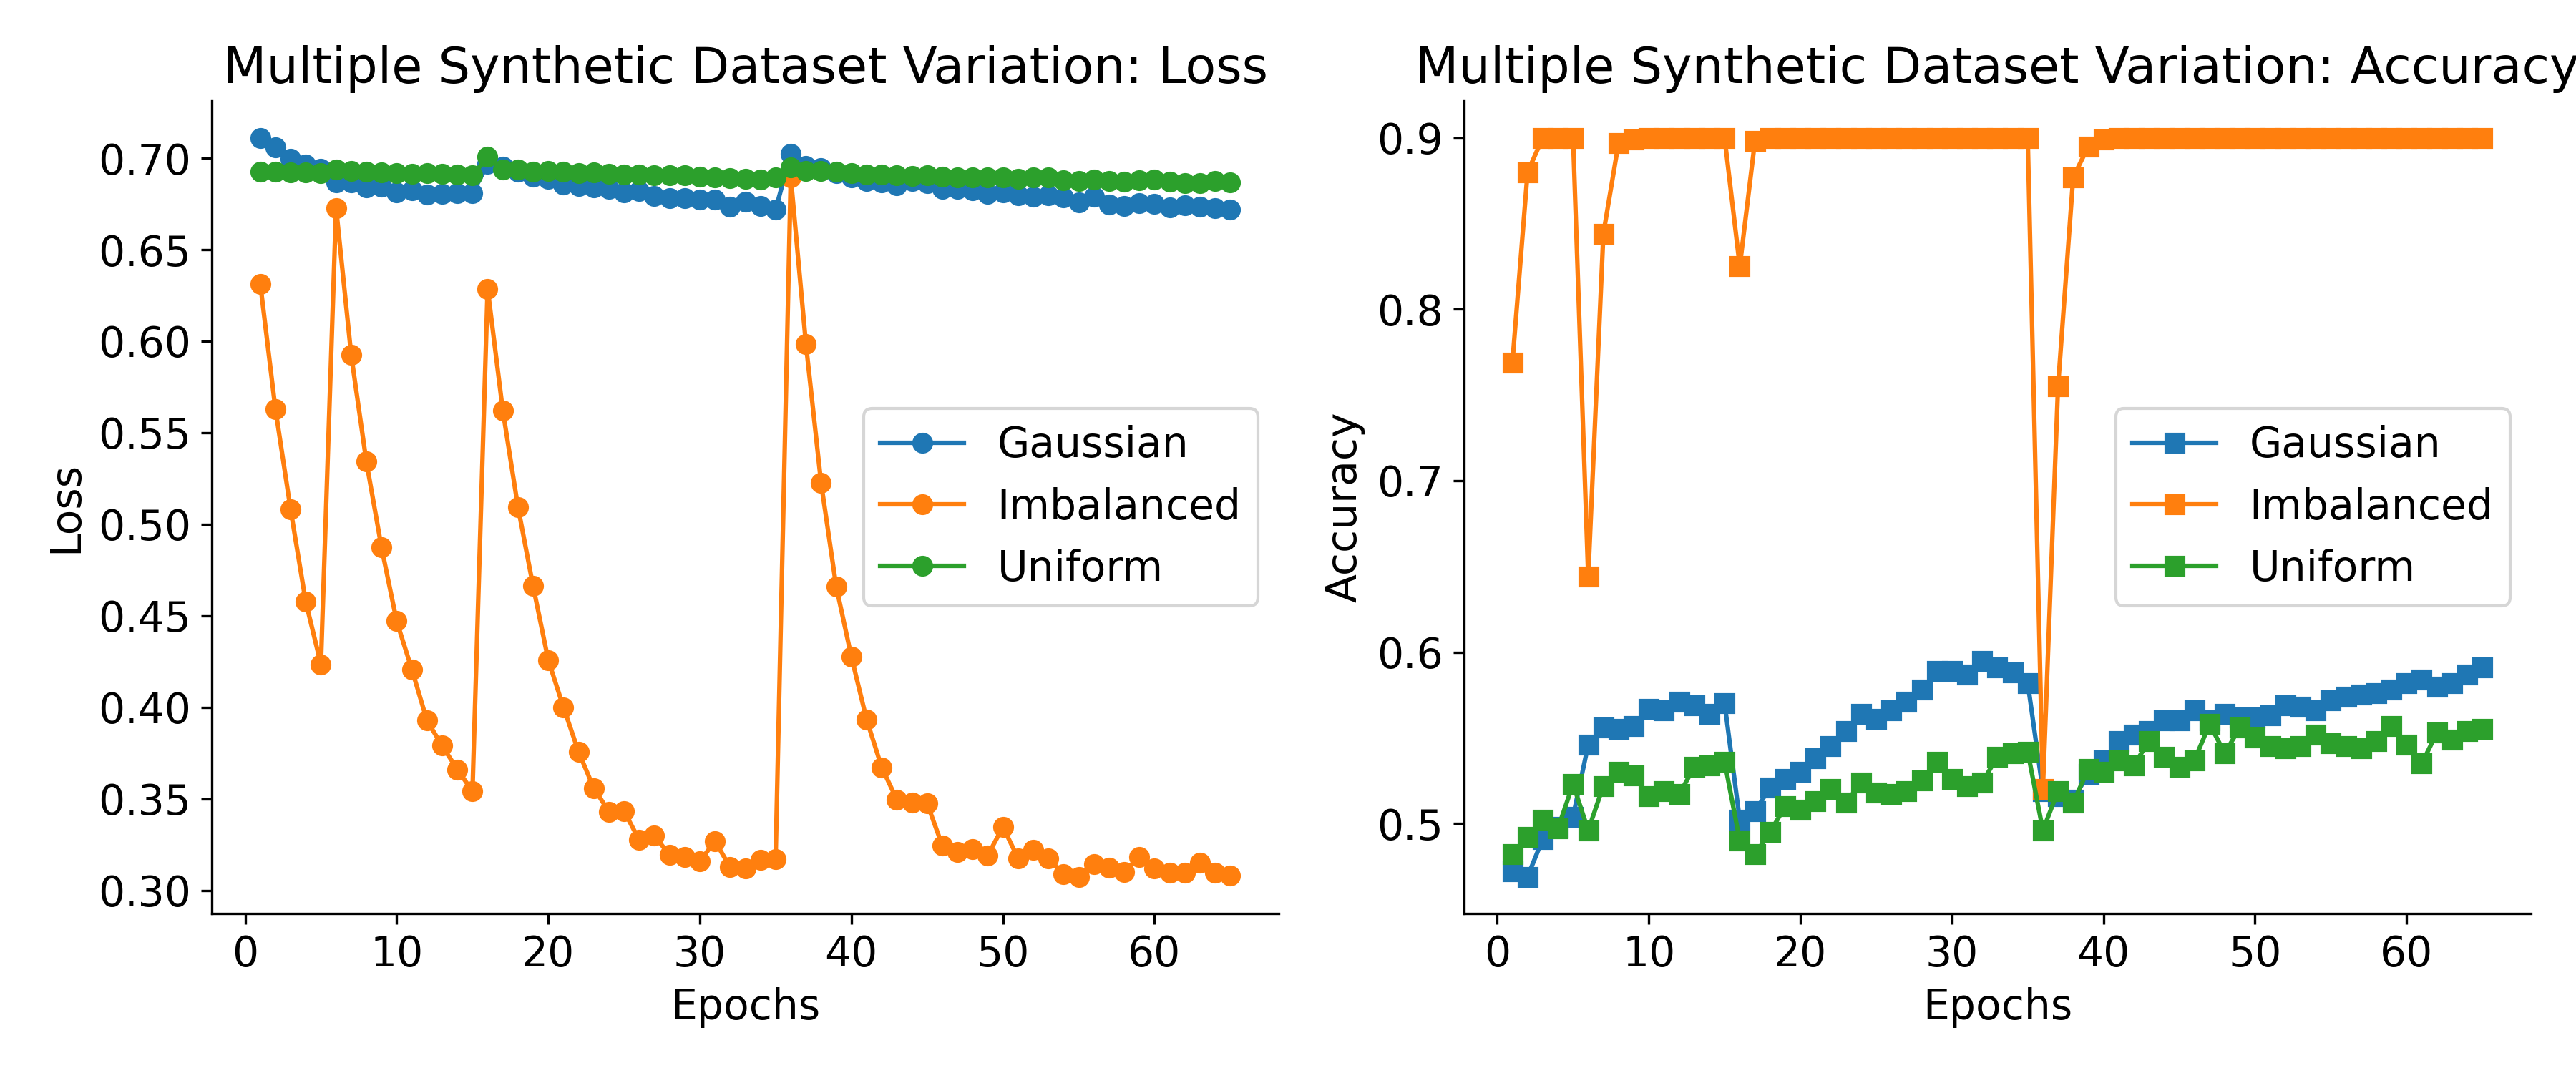
\includegraphics[width=0.48\textwidth]{multiple_synthetic_dataset_metrics.png}
\caption{Loss and accuracy over epochs for three synthetic datasets: Gaussian, Imbalanced, and Uniform. The Imbalanced dataset shows instability, while Gaussian and Uniform datasets exhibit stable performance.}
\label{fig:metrics}
\end{figure}

\begin{figure}[h!]
\centering
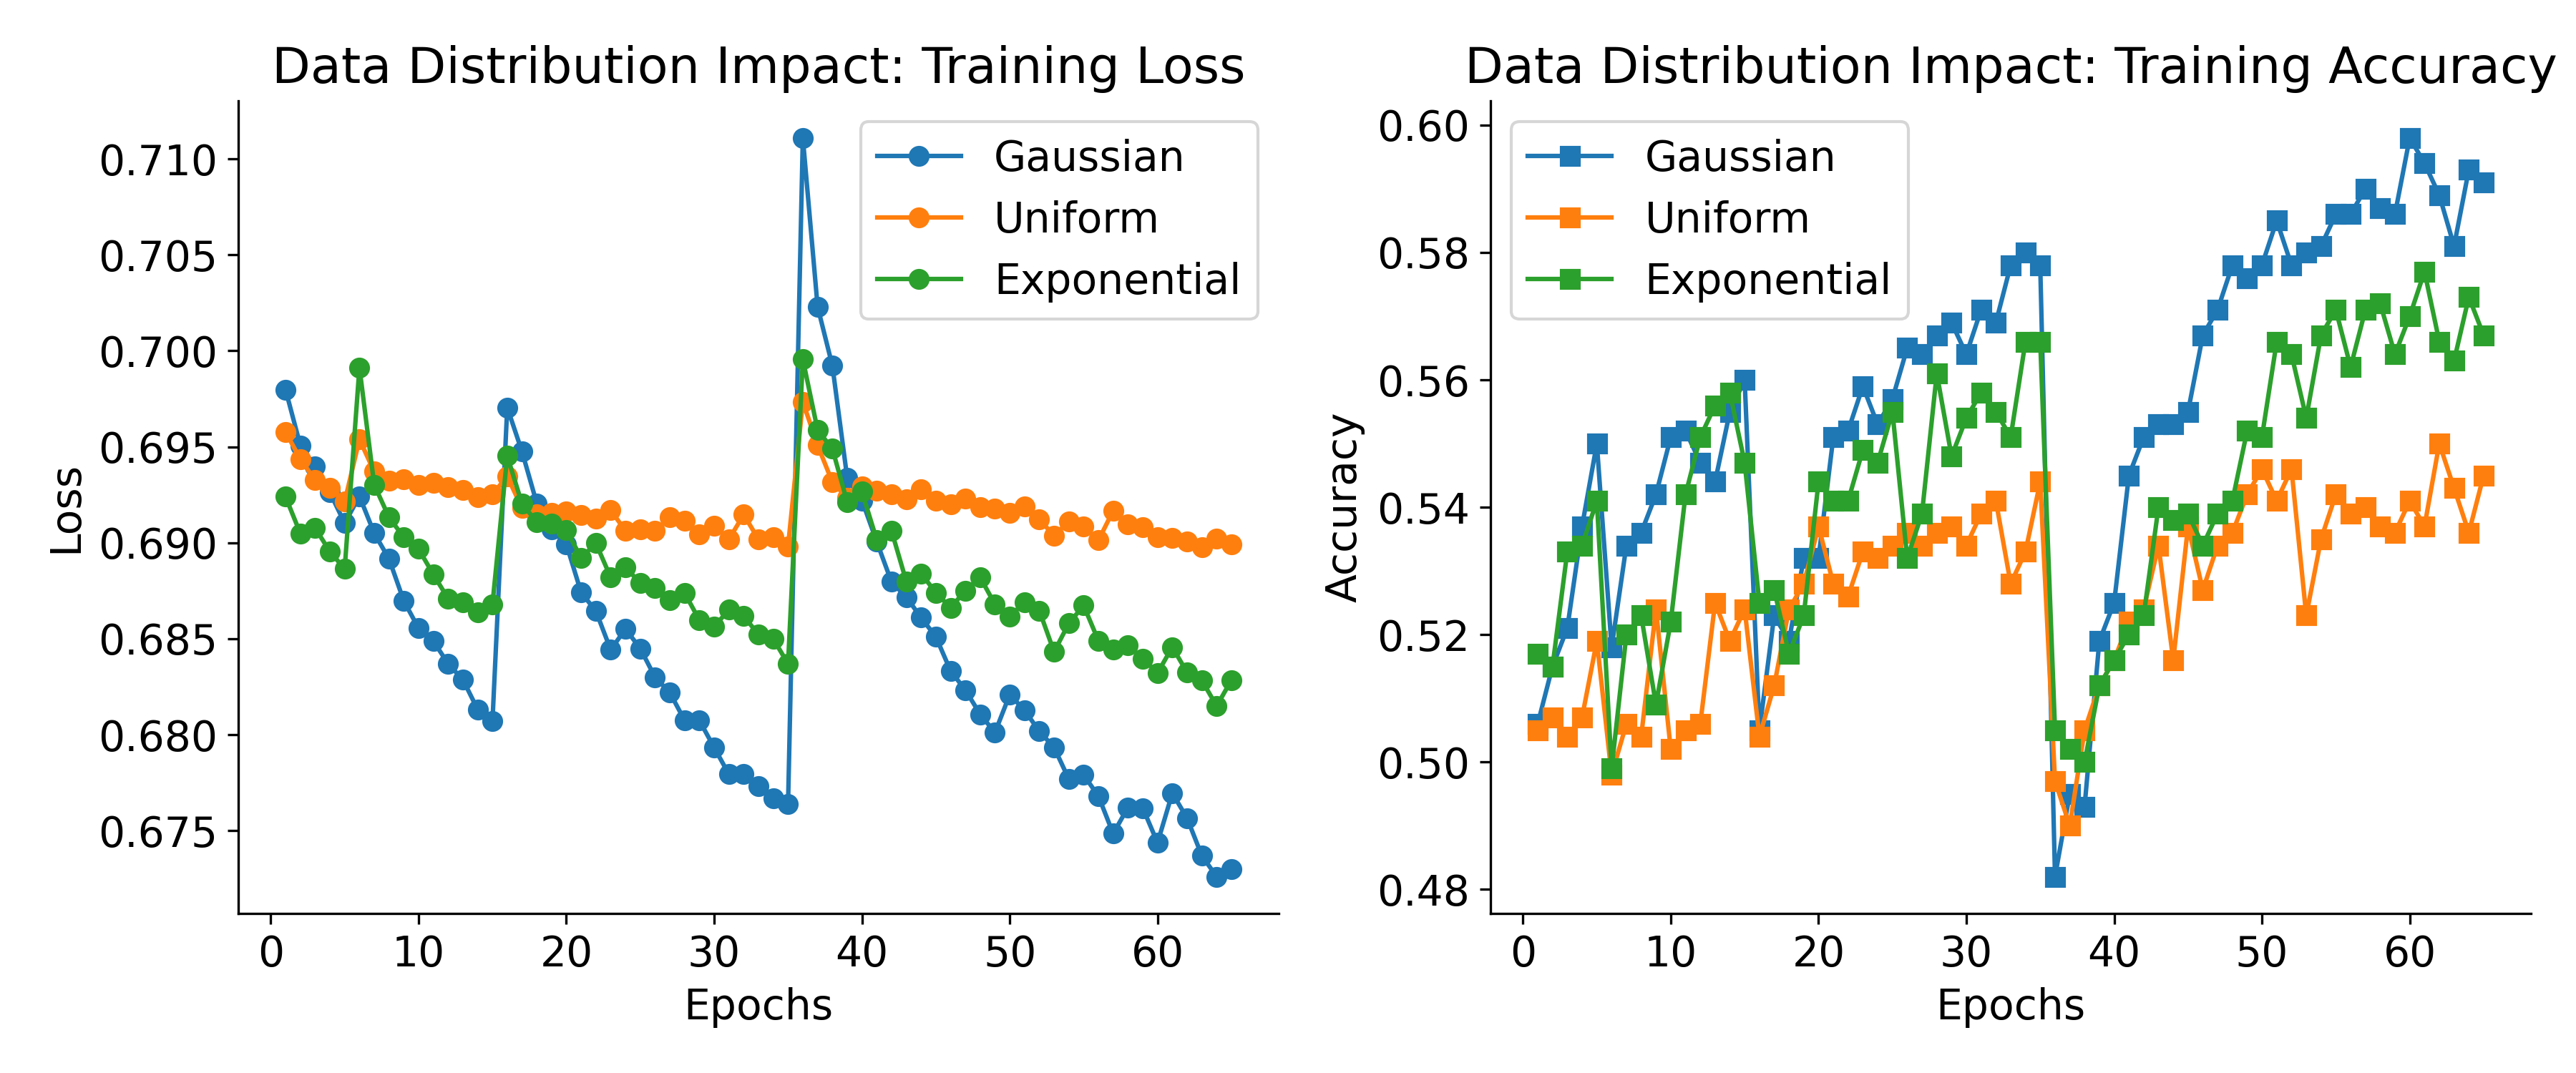
\includegraphics[width=0.48\textwidth]{data_distribution_impact.png}
\caption{Impact of different data distributions on training loss and accuracy. The Gaussian, Uniform, and Exponential distributions were analyzed across epochs, showcasing variances in model performance based on data characteristics.}
\label{fig:data_distribution}
\end{figure}

\begin{figure}[h!]
\centering
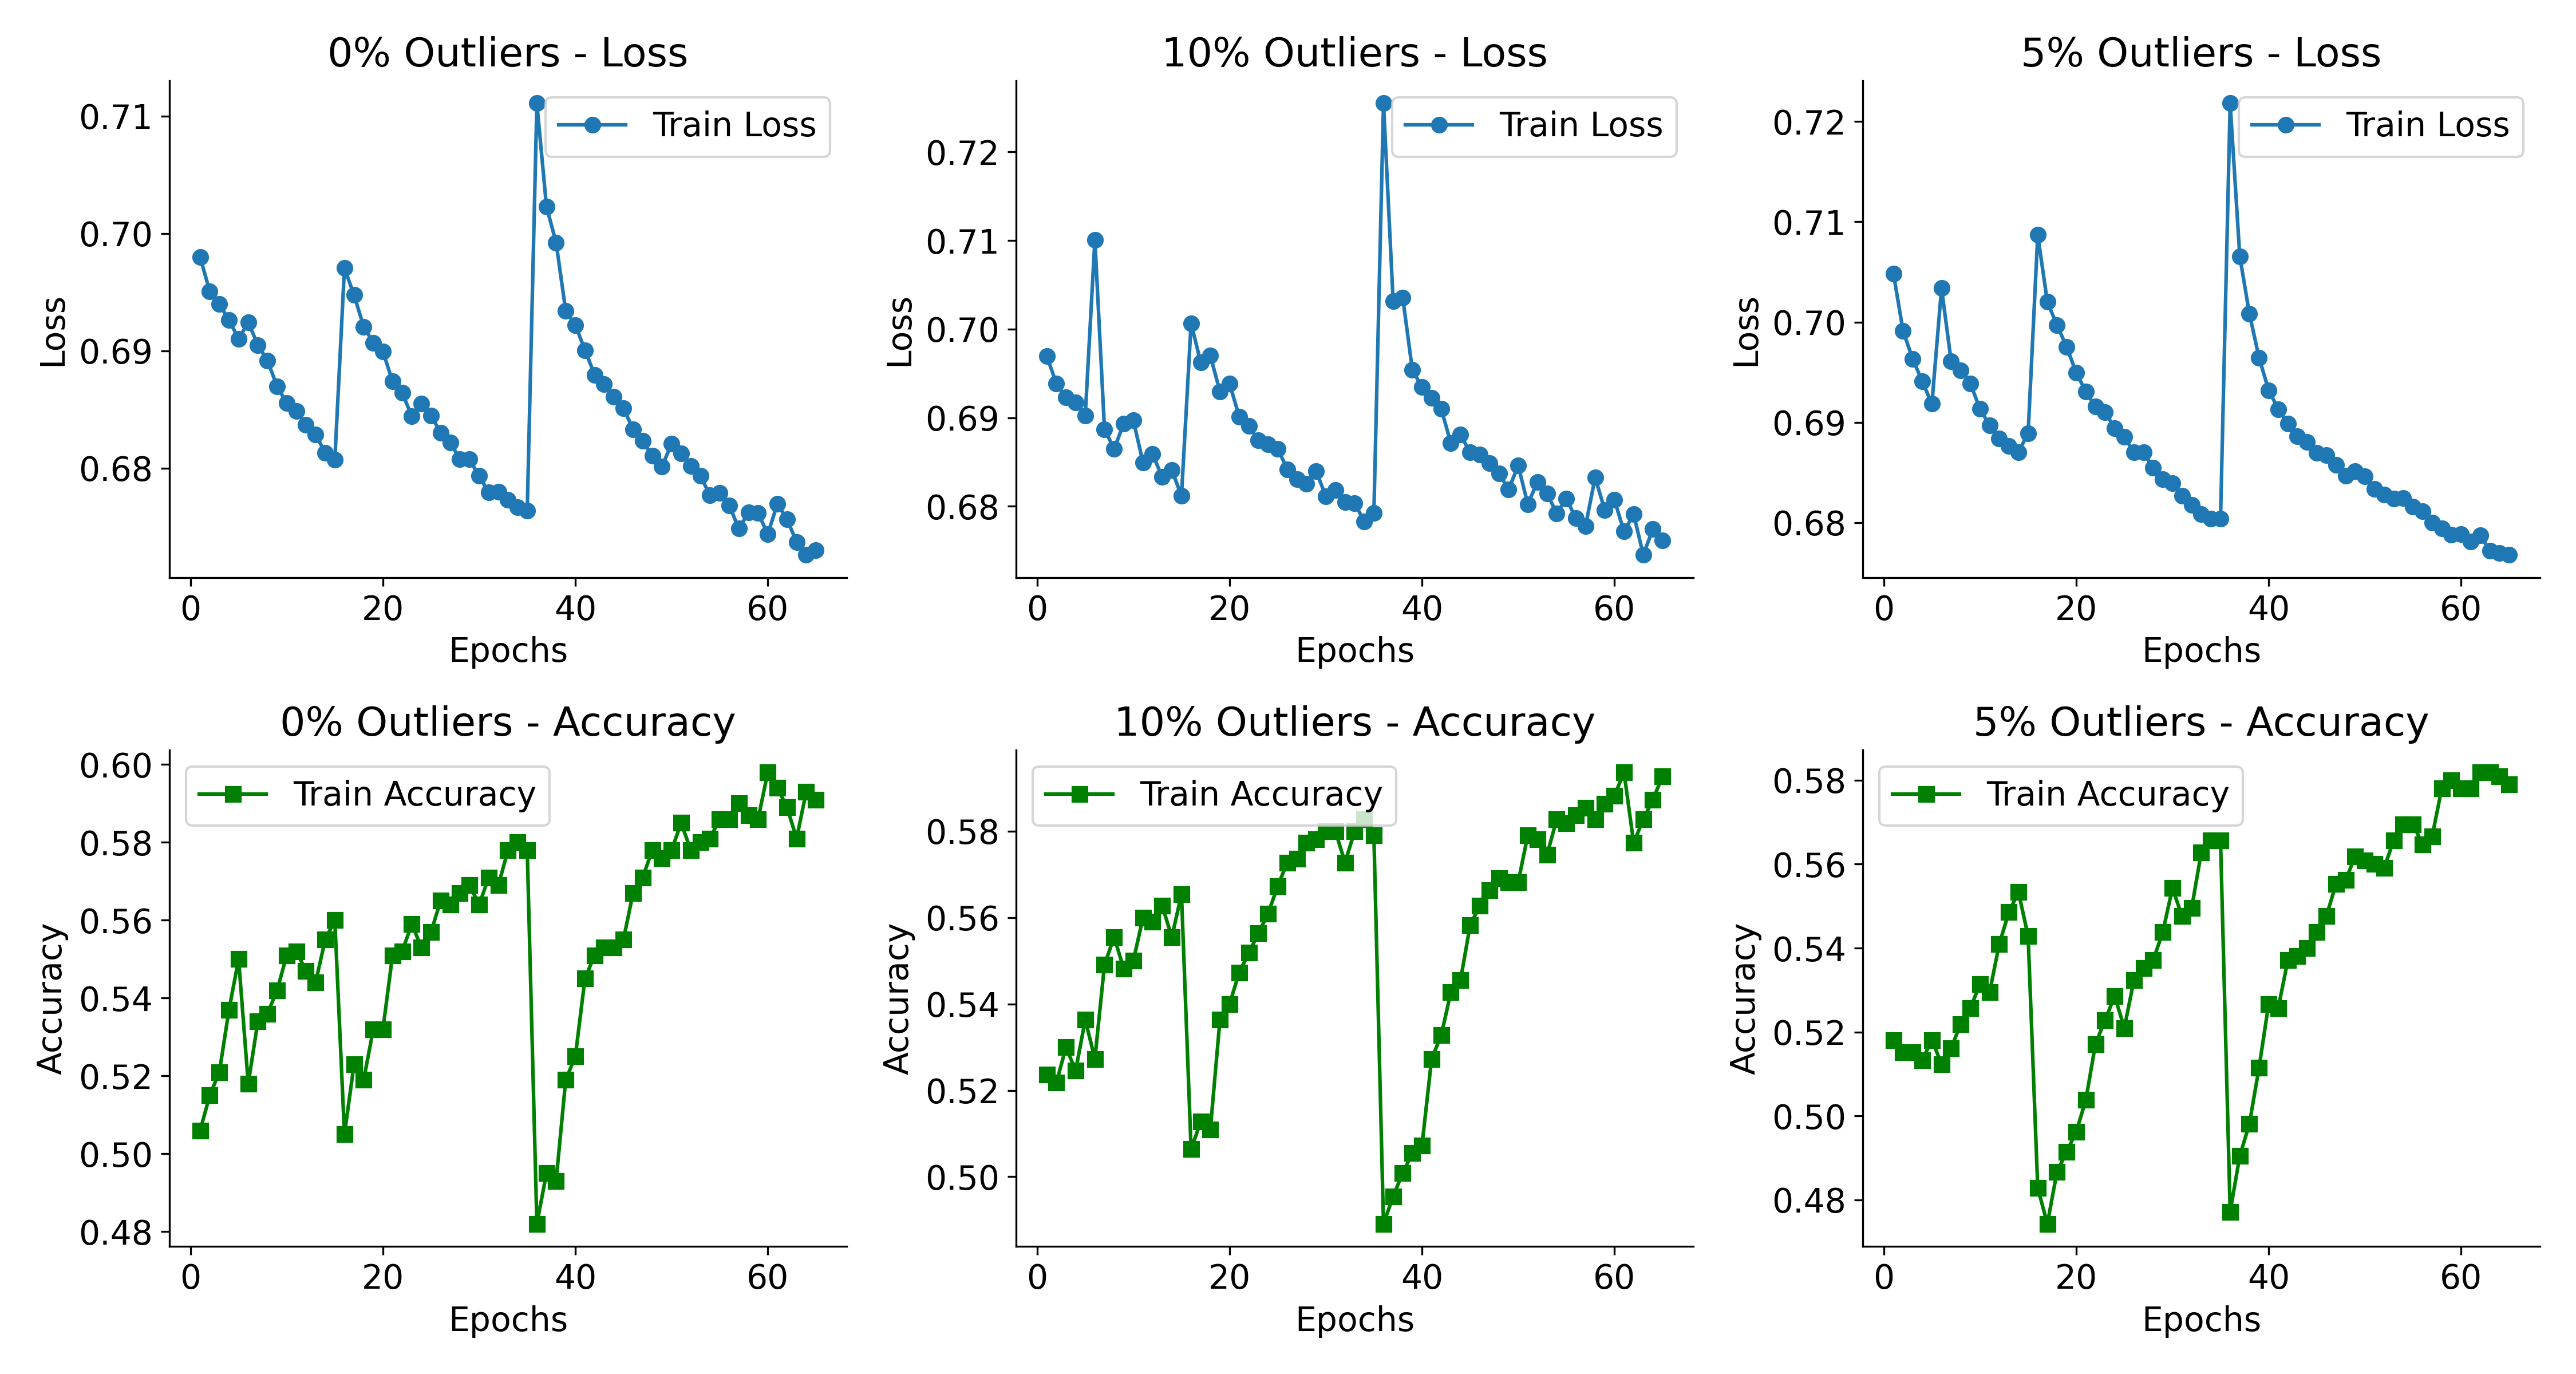
\includegraphics[width=0.48\textwidth]{outlier_impact_assessment.png}
\caption{Effects of varying outlier percentages on training loss and accuracy. The plots illustrate how different levels of outliers influence model stability and predictive performance.}
\label{fig:outlier_impact}
\end{figure}

\begin{figure}[h!]
\centering
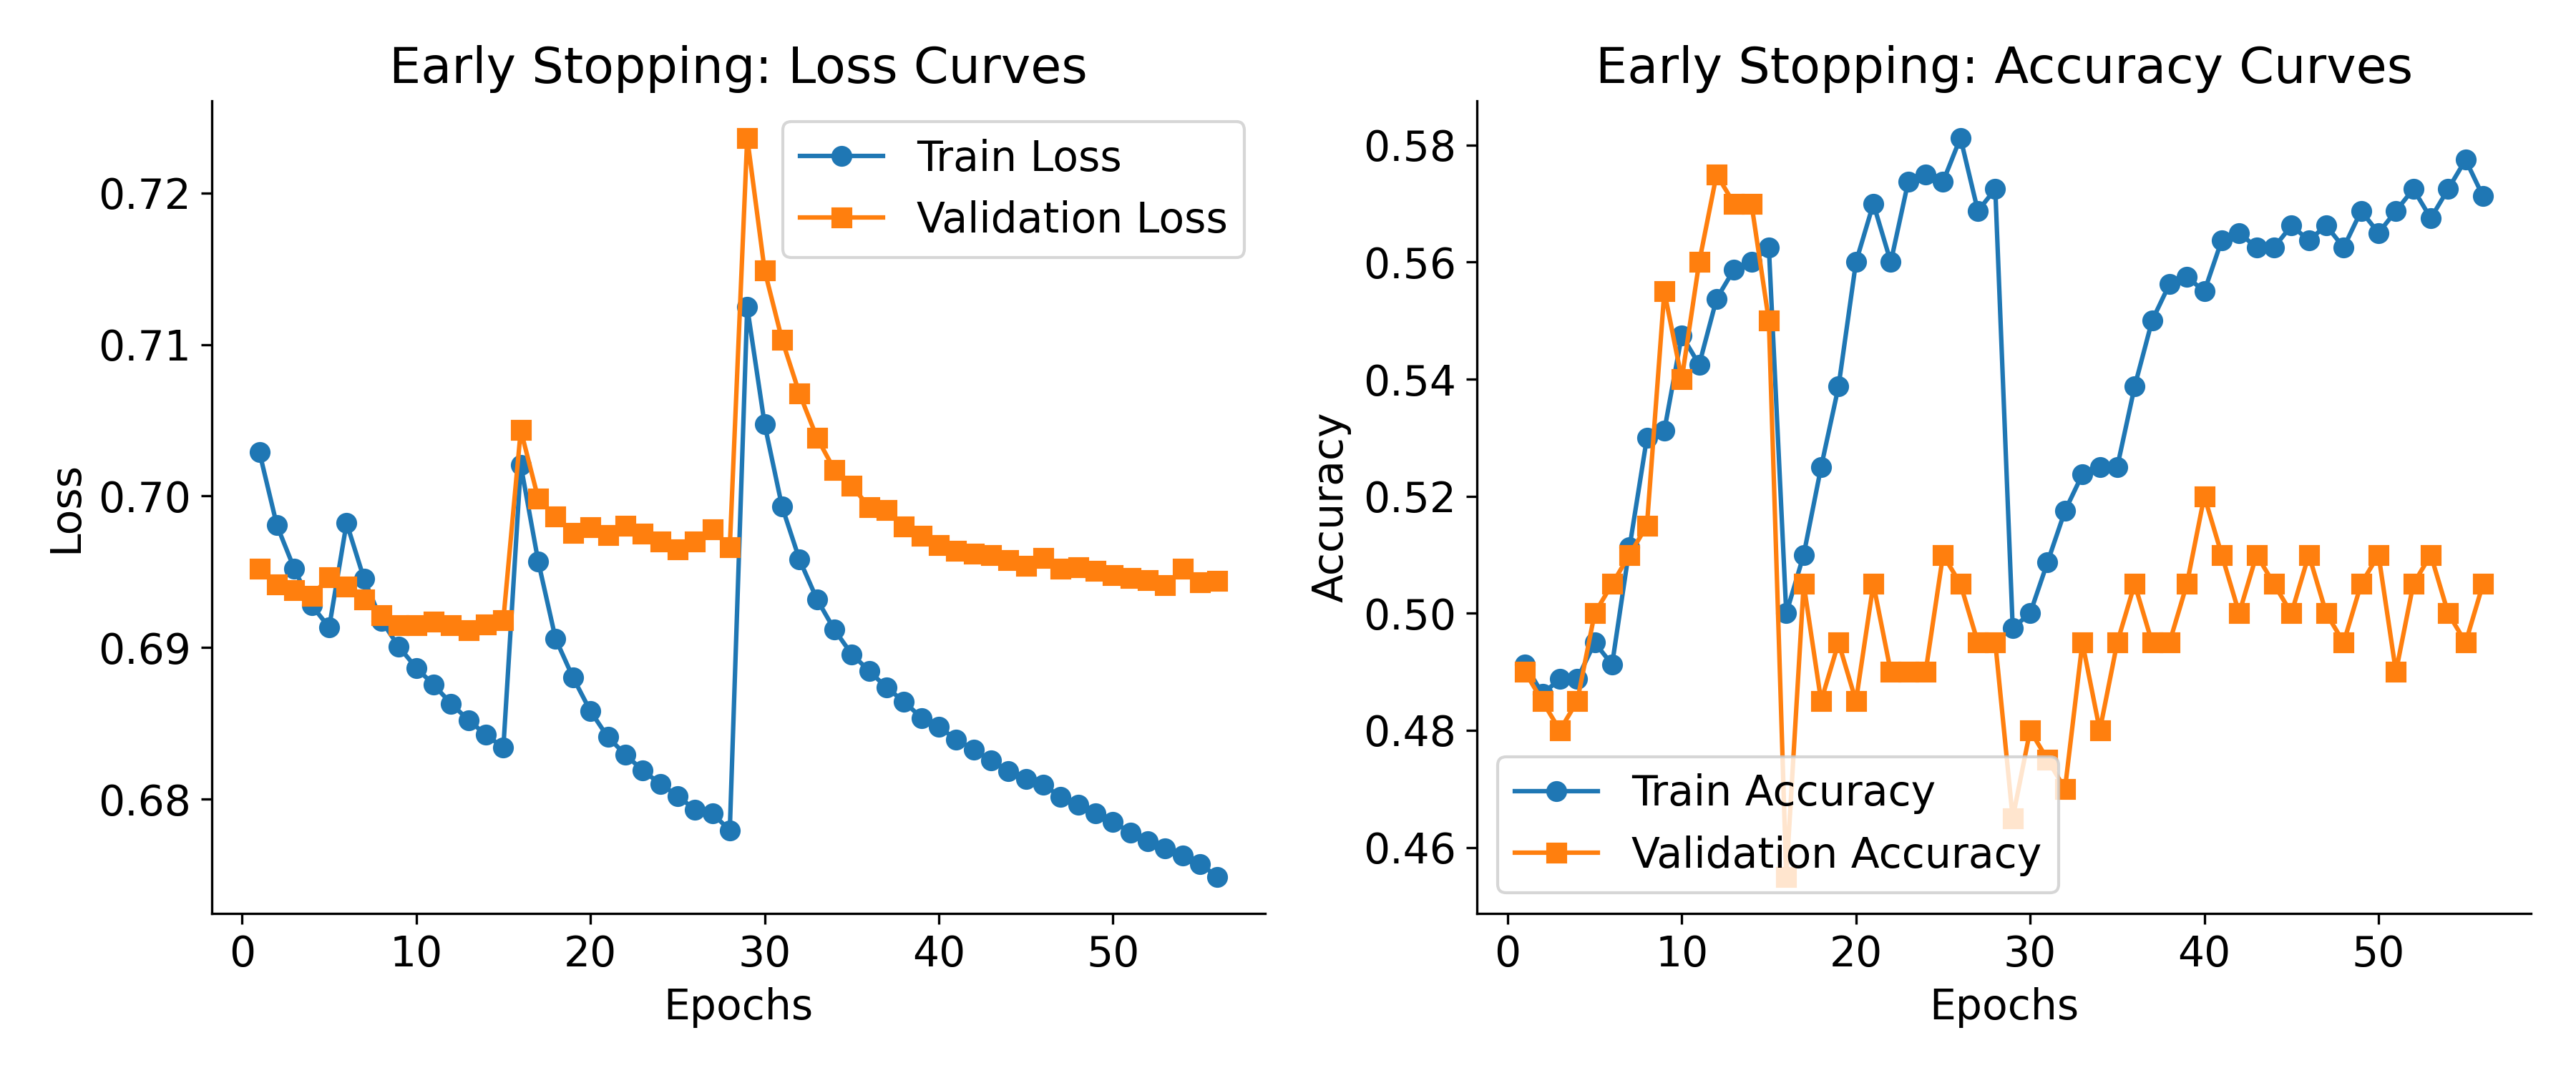
\includegraphics[width=0.48\textwidth]{early_stopping_mechanism.png}
\caption{Analysis of loss and accuracy curves under an early stopping mechanism, comparing training and validation performance throughout the epochs.}
\label{fig:early_stopping}
\end{figure}

The figures demonstrate that expanding screening capacity can yield substantial benefits in identifying vulnerable populations, even when predictive accuracy improvements are marginal. Notably, the Imbalanced dataset illustrated significant fluctuations in performance, emphasizing the importance of stability in model performance over absolute accuracy.

\section{Conclusion}
Our findings suggest that in resource-constrained settings, the trade-off between predictive accuracy and screening capacity is critical. By adopting the PAR framework, policymakers can make informed decisions about resource allocation that prioritize reaching vulnerable individuals effectively. Future work should further refine the PAR metric and explore its applicability in diverse social welfare contexts.

\bibliography{references}
\bibliographystyle{iclr2025}

\appendix
\section*{\LARGE Supplementary Material}
\label{sec:appendix}
The supplementary material includes additional details on the methodology, hyperparameter tuning, and further experimental results that support the findings presented in this paper.

\end{document}